
\label{ch:tests}

Test cases for CISM include experiments with analytic solutions, standardized experiments
without analytic solutions but for which community benchmarks are available, and
some experiments specific to CISM which have been well characterized by CISM developers.

Here we organize test cases based on the velocity solver that is most appropriate
for each test.  Any velocity solver can be used with any test
if the .config file settings are adjusted manually.  In some cases, however, the results
may be difficult to interpret.

Each test directory includes a README.md file with some technical details 
about how to run the test.  Many tests have python scripts that are used to set up
the initial condition and, in some cases, execute the model.  Some tests
have an additional python script for analyzing the CISM output.

The user must manually provide each test with access to the CISM executable.
There are several ways to do this:

\begin{itemize}
  \item Softlink the executable into the directory, e.g.:

        \texttt{ln -s ../../../builds/mac-gnu/cism\_driver/cism\_driver ./}

        This is the recommended procedure during development so that the test
        will always be using the most up-to-date version of the executable.

  \item Use the -e command line option to point to include an explicit path for the executable (for test case run scripts that support this option), e.g.:

        \texttt{./runDome.py -e ../../../builds/mac-gnu/cism\_driver/cism\_driver}

        This is useful for quickly trying a different version of CISM (e.g., comparing 
        serial and parallel executables).

  \item Add the directory containing the CISM executable to your environment PATH.

  \item Copy the executable into the directory.  This is typically not the most efficient approach,
        but may make sense in some situations.
\end{itemize}

The python scripts generally have useful
command line options that control their execution.  Typically, you can see details 
by using the \texttt{-{}-help} (or \texttt{-h}) command line option, e.g.:

\texttt{./runDome.py --help}

The various tests are described below.

% =====================================

\section{Shallow Ice Test Cases}

These tests are primarily useful for testing the shallow ice approximation (SIA) dycore, Glide.


% =====================================
\subsection{Halfar dome}
% =====================================

\label{sec:halfar_description}
This test case describes the time evolution of a dome of ice as described by \citet{Halfar1983}.
This test provide an analytic solution for a flat-bedded SIA problem.

\begin{equation}
    \label{halfar}
    \frac{\partial H}{\partial t} = \nabla \cdot (\Gamma H^{n+2} |\nabla H|^{n-1} \nabla H)
\end{equation}
where $n$ is the exponent in the Glen flow law, commonly taken as 3, and $\Gamma$ is a positive constant:
\begin{equation}
    \Gamma = \frac{2}{n+2} A (\rho g)^n
\end{equation}

For $n=3$, this reduces to:
\begin{equation}
    H(t,r) = H_0 \left(\frac{t_0}{t}\right)^\frac{1}{9}  \left[ 1 - \left(  \left( \frac{t_0}{t} \right) ^ \frac{1}{18} \frac{r}{R_0} \right)^\frac{4}{3} \right] ^ \frac{3}{7}
\end{equation}
where
\begin{equation}
    t_0 = \frac{1}{18\Gamma} \left( \frac{7}{4} \right)^3 \frac{R_0^4}{H_0^7}
\end{equation}
and $H_0, R_0$ are the central height of the dome and its radius at time $t=t_0$.

For more details see \url{http://www.projects.science.uu.nl/iceclimate/karthaus/2009/more/lecturenotes/EdBueler.pdf},  \citet{Bueler2005}, and \citet{Halfar1983}.



\subsubsection{Provided Files}
\label{subsec:halfar_files}

Our implementation of the Halfar dome has an initial radius of $R_0=21.2$ km and an initial thickness of $H=707.1$ m.
These values can be changed by editing \texttt{halfarDome.py}.

\begin{itemize}
	\item README \\
		Information about the test case, including technical details about running it.
	\item halfar.config \\
		This is the config file defining CISM options. \\
    There is also a version named \texttt{halfarHO.config} that is setup to run the Glissade dycore.
	\item halfar.py \\
		This python script generates the dome initial condition and \\
		runs CISM.
	\item halfar\_results.py \\
		This is script compares model results to the analytic solution.
	\item halfarDome.py \\
		This is a python module that defines the analytic solution. \\
    It is not meant to be run manually, but it is imported by the other scripts.
\end{itemize}

\subsubsection{Running the test}
One script sets up the initial condition and runs the model:

\texttt{./halfar.py}

Another script analyzes the results:

\texttt{halfar\_results.py}

\subsubsection{Results}
\label{subsecc:halfar_results}
With the default .config settings, this simulation should only take a few seconds and is a good first test for a working Glide dycore.
As the dome of ice evolves, its margin advances and its thickness decreases (there is no surface mass balance to add new mass).  The script \texttt{halfar\_results.py} will plot the modeled and analytic thickness at a specified time (Figure \ref{fig:halfarresults}), as well as report model error statistics.  Invoke \texttt{halfar\_results.py --help} for details of its usage.


\begin{figure}[H]
	\centering
	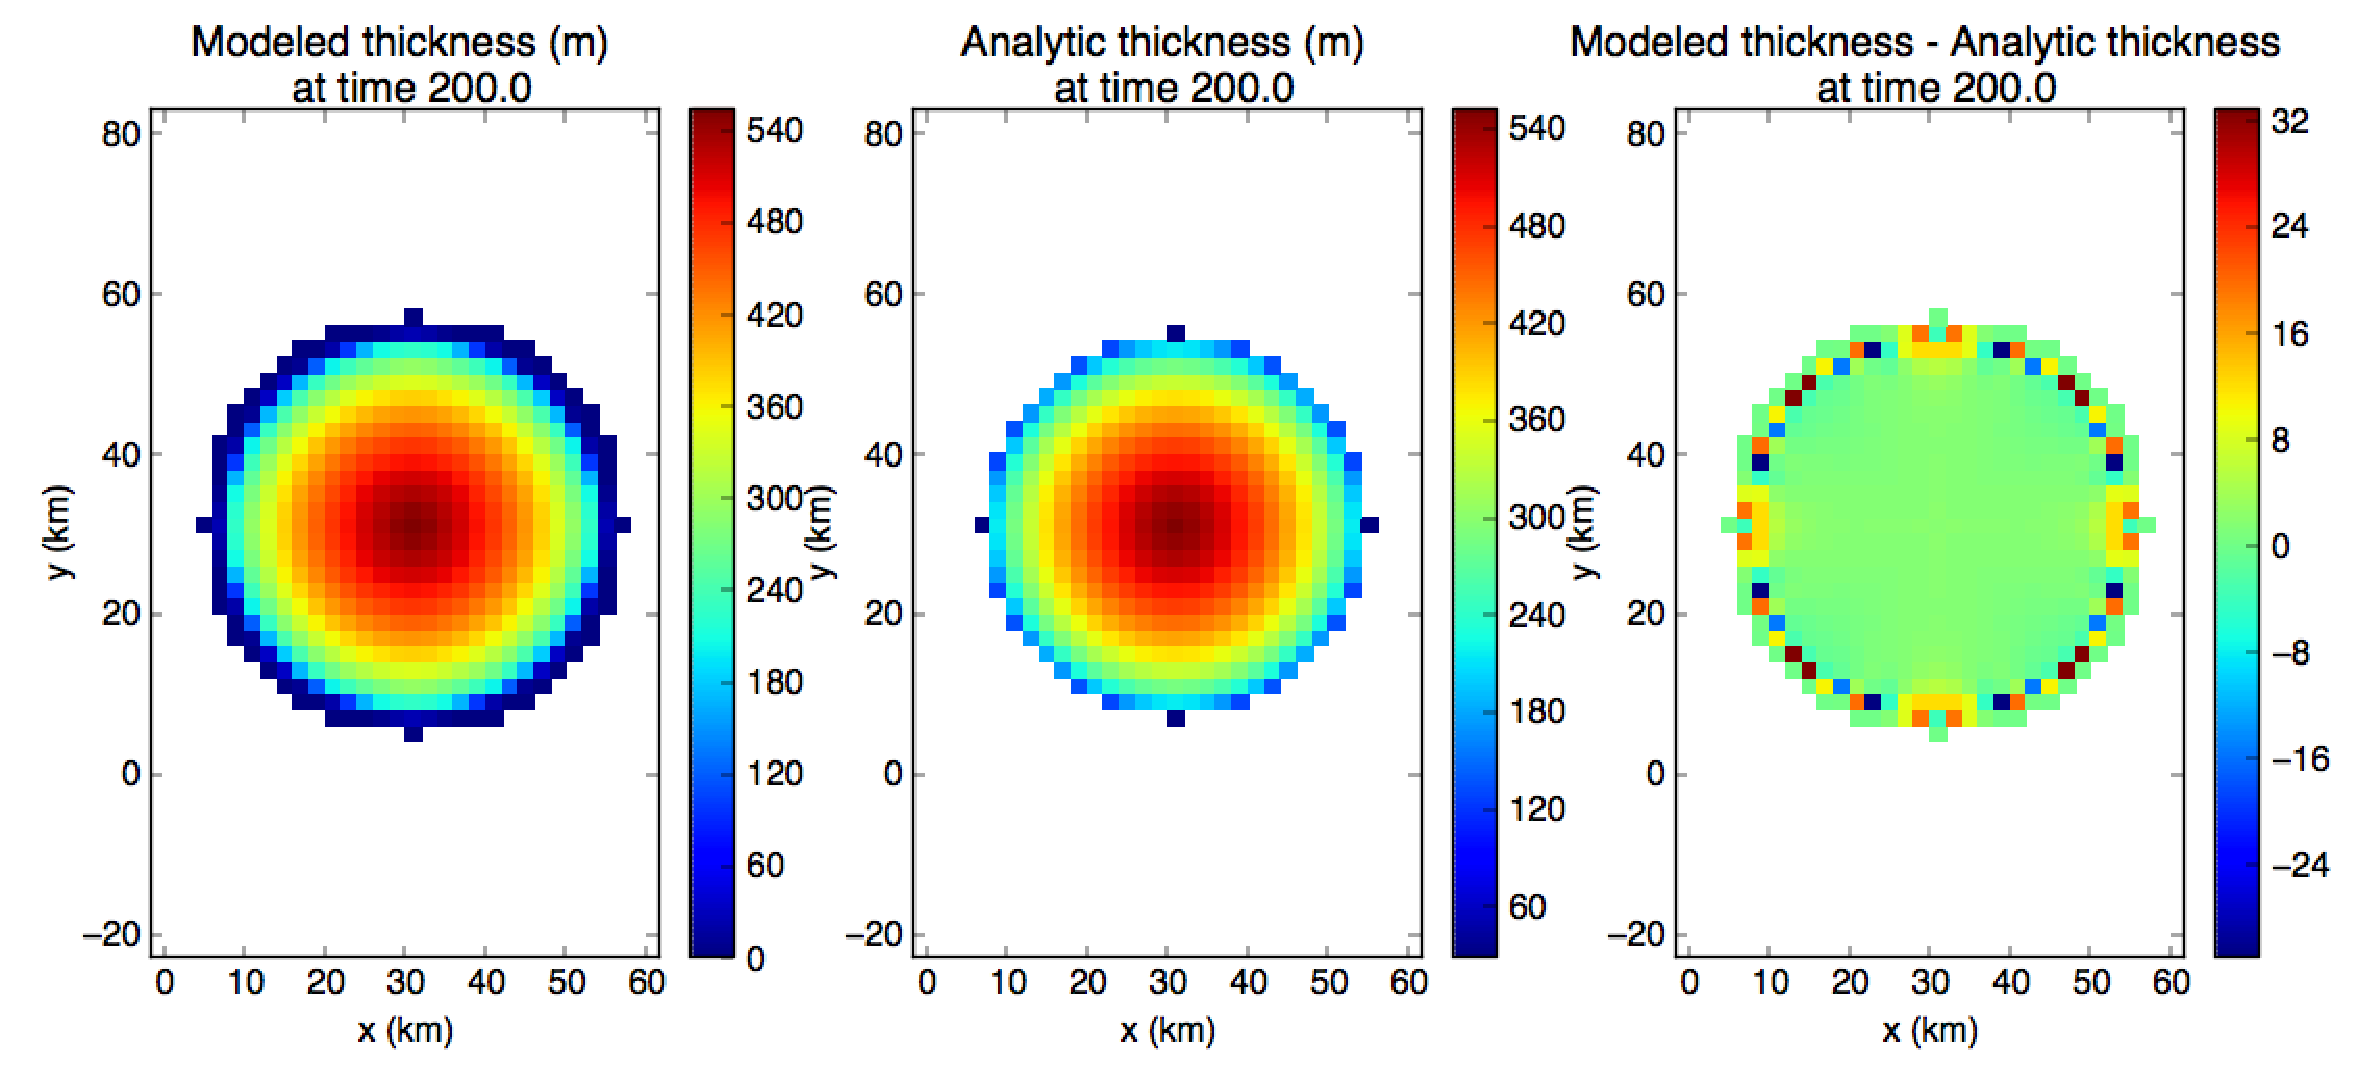
\includegraphics[width=16.4cm]{\dir/halfar_results.eps}
	\caption{Halfar test case results after 200 years of dome evolution. This figure is generated by \texttt{halfar\_results.py}.}
	\label{fig:halfarresults}
\end{figure}


\FloatBarrier


% =====================================
\subsection{EISMINT-1}
% =====================================
\label{sec:eismint_description}
This test case is from phase 1 of the European Ice Sheet Modelling INiTiative intercomparison experiments.  These experiments are described at \url{http://homepages.vub.ac.be/~phuybrec/eismint.html} and in \citet{Huybrechts1996}.

\subsubsection{Provided Files}
\label{subsec:eismint_files}

\begin{itemize}
	\item README \\
		Information about the test case, including technical details about running it.
\item *.config \\
  There are six .config files for each of the six experiments in EISMINT 1.  There are three fixed margin experiments (fm) and three moving margin experiments (mm).
\end{itemize}

\subsubsection{Running the test}
There is not a script for running these experiments.  They must be run manually, e.g.: 

\texttt{./cism\_driver e1-fm.1.config}


\subsubsection{Results}
\label{subsecc:eismint_results}
These experiments are meant to be run to steady-state, and the supplied .config files are setup to run for long enough for it to be reached.
These simulations take more than a few minutes to complete.
As the initial ice sheet evolves, its shape eventually reaches a steady-state with the imposed surface mass balance.  Currently there is not a script for analyzing the CISM results.  Users can manually compare their results to those in the \citet{Huybrechts1996} paper.


% =====================================
\subsection{EISMINT-2}
% =====================================
\label{sec:eismint2_description}
This test case is from phase 2 of the European Ice Sheet Modelling INiTiative intercomparison experiments.  These experiments are described at \url{http://homepages.vub.ac.be/~phuybrec/eismint.html} and in \citet{Payne2000}.

\subsubsection{Provided Files}
\label{subsec:eismint2_files}

\begin{itemize}
	\item README \\
		Information about the test case, including technical details about running it.
  \item *.config \\
  There are 11 .config files for each of the a-f experiments in EISMINT-2.
  \item mound.nc, trough.nc \\
    These are input netCDF files used by the EISMINT-2 experiments.
\end{itemize}

\subsubsection{Running the test}
There is not a script for running these experiments.  They must be run manually, e.g.: 

\texttt{./cism\_driver e2.a.config}


\subsubsection{Results}
\label{subsecc:eismint2_results}
These experiments are meant to be run to steady-state, and the supplied .config files are setup to run for long enough for it to be reached.  
Note that some of the experiments use the final state of a previous experiment 
as the initial condition.  See experiment descriptions in \citet{Payne2000} for details.
These simulations take more than a few minutes to complete.
As the initial ice sheet evolves, its shape eventually reaches a steady-state with the imposed surface mass balance.  Currently there is not a script for analyzing the CISM results.  Users can manually compare their results to those in the \citet{Payne2000} paper.


% =====================================
\subsection{GLINT example}
% =====================================
Glint example description

\subsubsection{Provided Files}

\begin{itemize}
	\item README \\
		Information about the test case, including technical details about running it.
\item ?.config \\
  ???
\item ???... \\
\end{itemize}

\subsubsection{Running the test}
There is not a script for running this experiment.  It must be run manually, e.g.: 

\texttt{./cism\_driver greenland\_20km.config glint\_example.config}

[describe the two .config syntax]

\subsubsection{Results}
???




% =====================================

\section{Higher-Order Test Cases}

Info here about running the various HO test cases.

\subsection{Dome}

\subsection{ISMIP-HOM}

\subsection{Confined Shelf}

\subsection{Circular Shelf}

\subsection{Ross Ice Shelf}


